\chapter{Grundlagen und Stand der Technik}

Für den Prozess der Deformationserkennung sind grundlegende Kenntnisse der 
Additiven Fertigung sowie des 3D-Designs von Vorteil. In diesem Kapitel 
werden sowohl diese Grundlagen als auch der aktuelle Stand der Technik 
erläutert.

\section{Additive Fertigung}

Additive Fertigung (AF) ist unabhängig von dem Werkstoff ein Bereich, in dem viel
geforscht und innoviert wird. In fast jedem Industriebereich wird versucht, ein
bestehendes Design oder Modell zu optimieren und zu verbessern.
Sei es hinsichtlich Qualität oder Kosteneffizienz. AF bietet bei 
dieser Optimierung viele Vorteile gegenüber spanenden Fertigungsverfahren, da 
AF einen höheren Grad der Gestaltungsfreiheit bietet. \cite{durakovic2018design}
AF ist eine Ressource, welche Benutzern ermöglicht, komplexe 
Bauteilgeometrien zu erstellen, ohne die Limitierung von konventionellen spanenden 
Herstellungsverfahren zu erstellen. 
Limitierungen von konventionellen spanenden 
Herstellungsverfahren kann ein hoher Materialverschleiß oder die Notwendigkeit von 
spezialisierten Werkzeugen sein.\ \cite{Vafadar.2021} 

Außerdem können mit additiver Fertigung Stückzahlen drastisch reduziert werden.
Werkstücke können bei Bedarf gefertigt werden, was die Notwendigkeit für Lagerstätten
größtenteils eliminiert. Zusätzlich können die Teile genau dort herstellt werden, wo 
sie benötigt werden, was Lieferketten und Wartezeiten verkürzt~\cite{Calignano.2023}.

Bauteile können mit verschiedenen Werkstoffen, darunter sind Polymeren, Metalle und Keramik, 
additiv gefertigt werden.
Metalle haben vor allem in den letzten Jahren 
an Relevanz gewonnen. Zusätzlich zu den schon genannten Vorteilen von AF, 
bietet Metall als Werkstoff großen Nutzen in der Industrie. Gegenüber Kunststoffen
produziert Metall weniger Abfall und kann eine höhere Qualität gewährleisten.
Zusätzlich dazu kommen die offensichtlichen Vorteile von Metall gegenüber Polymeren: 
höhere Hitzebeständigkeit und eine stabilere Grundstruktur, was sie weniger anfällig 
für Verformungen macht~\cite{Gardner.2023}.

Aufgrund dieser Vorteile wird AF in vielen Industriebereichen genutzt. 
Beispielsweise die Automobilbranche ist ein Bereich, in der AF schon viel und erfolgreich 
eingesetzt wird:
Durch AF könne Teile gefertigt werden, die leichter, belastbarer und sicherer sind. 
Die einfache Anpassbarkeit sorgt für geringe Entwicklungszeiten und Kosten. 
BWM benutzt für den i8 Roadster viele AF gefertigte Teile.
Darunter sind zum Beispiel die Befestigung für das Soft-Top, die 44 \% leichter als das Spritzgussteil
ist, und dennoch zehnmal steifer.\ \cite{Vafadar.2021} 
Fensterführungen wurden auch additiv gefertigt. Mithilfe des \glqq HP Multi Jet Fusion\grqq~
konnten 
100 Teile in 24 Stunden gefertigt werden. Selbst Teile des Zylinderkopfs für den 
S58 Motor wurden additiv gefertigt. \cite{Anusci.2019}

Auch bei älteren Fahrzeugen können additive Fertigungsmethoden zur 
Reparatur oder Restauration verwendet werden.
Gerade bei älteren Fabrikaten sind Ersatzteile häufig nicht mehr vom 
Erstzulieferer zu beschaffen oder mit konventionellen Herstellungsmethoden
wirtschaftlich herzustellen.
Bei einem Matra 530 aus 1973 wurde zum Beispiel die rechte 
Kotflügelhalterung erfolgreich reproduziert, nachdem auch nach längerer Suche
kein Originalteil gefunden wurde \cite{AMExpo365.03.06.2024}. Zusätzlich war
bei diesem Beispiel die Herausforderung, das keine digitale Version des
Bauteils existiert hat. Zuerst musste also ein Modell als Grundlage für die
additive Fertigung erzeugt werden.

\section{Limitierungen von AF}

AF kann trotz seiner Vorteile nicht überall eingesetzt werden. Limitierungen 
in der Materialvielfalt, hohe Material und Anschaffungskosten, begrenzte
Bauraumgrößen, verminderte Oberflächenqualität und aufwändige Nachbearbeitungen
können einen Einsatz von AF verhindern beziehungsweise unwirtschaftlich machen. 
\cite{inproceedings}

Einige dieser Limitierungen können umgangen oder gelöst werden. 
Zum Beispiel kann die
verminderte Oberflächenqualität durch eine anschließende Fräsbearbeitung
verbessert werden. 
Diese Nachbearbeitung macht eine Fixierung des Bauteils notwendig. Auch für andere
Nachbearbeitungen wie das Entfernen von Stützstrukturen kann sich das fixieren
positiv auswirken und Zeit im Herstellungsprozess eingespart werden.
Wie schon in Kapitel \ref{drawbacks_af} beschrieben, sind 
Stützstrukturen notwendig, wenn das zu produzieren Bauteil Überhänge aufweist,
die eine Steigung von ungefähr 30° unterschreiten. In Abbildung \ref{fig:overhang}
ist ersichtlich, warum Stützstrukturen bei einigen Bauteilgeometrien notwendig
sind. Der Grad des Überhangs, der ohne Stützstrukturen hergestellt werden kann,
variiert je nach verwendetem Material und Verfahren.~\cite{Meng.2020} 

\begin{figure}[H]
    \centering
    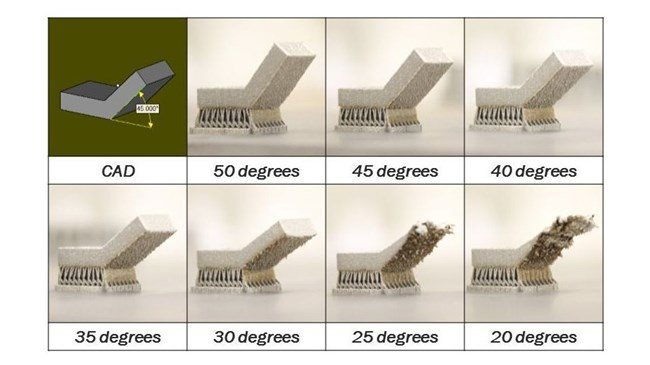
\includegraphics[width=0.9\linewidth]{images/Overhang-tests-showing-different-printabilities-and-finish-qualities-at-seven-different.jpg}
    \caption{Überhangtests mit unterschiedlichen Resultaten und 
    Oberflächenqualitäten in sieben verschiedenen Winkeln \cite{Meng.2020}}
    \label{fig:overhang}
\end{figure}

\section{Reverse Engineering}

Reverse Engineering beschreibt den Prozess aus einem bestehenden Produkt 
oder Objekt ein digitales Abbild zu erzeugen. Das im Rahmen dieser Arbeit
zu entwickelnde Verfahren ist im Prinzip ähnlich, 
da auch von einem bestehenden Bauteil eine digitale Version
erzeugt werden soll. Aufgrund des ähnlichen Prinzips ist der Prozess des Reverse Engineering
eine wichtige Grundlage dieser Arbeit.
Beim Reverse Engineering sind meistens wenig oder keine technischen Details
über das Objekt verfügbar.~\cite{Helle.2021}

Auch wenn Baupläne vorhanden sind, kann es trotzdem notwendig sein, 
Reverse Engineering zu betreiben, denn das tatsächliche Produkt kann von
den Bauplänen abweichen. Produkte und Bauteile können durch die Verwendung 
abgenutzt werden und entsprechen deswegen unter Umständen nicht mehr den originalen 
Bauplänen. Zusätzlich können Toleranzen im ursprünglichen Fertigungsprozess 
für Diskrepanzen sorgen. Wenn technische Details vorhanden sind,
können diese aber im Reverse Engineering Prozess verwendet werden. 
Reverse Engineering kann genutzt werden, um 
bestehende Bauteile passgenau zu erweitern. Ein Beispiel hierfür ist, die
Entwicklung einer Methodik um automatisiert Laser-Scans und originale Baupläne
zusammenzufügen um ein möglichst detailgetreues Abbild der realen Struktur zu
erzeugen. Dieses Abbild kann dann benutzt werden, um eine bestehende Struktur zu 
erweitern und auf ihr aufzubauen. S. Mönchinger demonstriert dies am Beispiel eines 
Flugzeugs. Zunächst wird der Innenraum gescannt und mit den originalen Plänen abgeglichen, 
um anschließend ein 3D-Modell zu erstellen. Mithilfe dieses 3D-Modells können passgenaue 
Bauteile hergestellt werden, die es ermöglichen, ein ehemaliges Passagierflugzeug in eine 
Frachtmaschine umzubauen.~\cite{Monchinger.2021}
Wie schon erwähnt, wird zur erfolgreichen Weiterbearbeitung ein möglichst 
genaues digitales Abbild benötigt.
Ist dies nicht der Fall, müssen nicht passende Teile erneut hergestellt werden, 
was die Material- und Personalkosten deutlich erhöht. Es ist also im 
wirtschaftlichen Interesse beim ersten Schritt, dem Erstellen der digitalen 
Version, ein möglichst genaues Ergebnis zu erzielen. 

\section{Digitales Abbild}

Für die weitere Verarbeitung ist es von notwendig, dass die erstellten digitalen 
Abbilder in einem geeigneten Datenformat gespeichert werden. Ansprüche hierbei sind 
eine, dem Nutzungszweck angepasste, realitätsnahe Abbildung der Objektgeometrie, 
ohne eine praktikable Dateigröße zu überschreiten.
Für diese effiziente Speicherung digitaler Abbilder haben sich mehrere
Dateiformate etabliert.
Die Geometrie eines Objekts wird häufig als Sammlung von Punkten 
gespeichert. Die Oberfläche eines Objekts wird als Serie von Polygonen beschrieben. 
Der Grad des Polygons kann variieren, häufig werden Dreiecke verwendet. \cite{lee2019study}

Die Genauigkeit, mit der das Polygon-Netz die gewünschte Oberfläche 
abbildet, kann gewählt werden. 
Je kleiner die Oberfläche der Polygonen ist, desto genauer wird die Oberfläche 
abgebildet. Mit kleineren Oberflächen steigt die Anzahl der zu speichernden 
Eckpunkte, was eine größere Datei zur Folge hat.
In Abbildung \ref{fig:3d_design} ist der Einfluss der Oberflächengröße der Polygonen
auf die gespeicherte Bauteilgeometrie zu sehen. Bei kleinen Polygonen 
wird die reale Bauteilgeometrie abgebildet. Umso weniger Polygone gespeichert 
werden, umso kantiger wird das Modell.

\begin{figure}[H]
    \centering
    \begin{minipage}{0.32\textwidth}
        \centering
        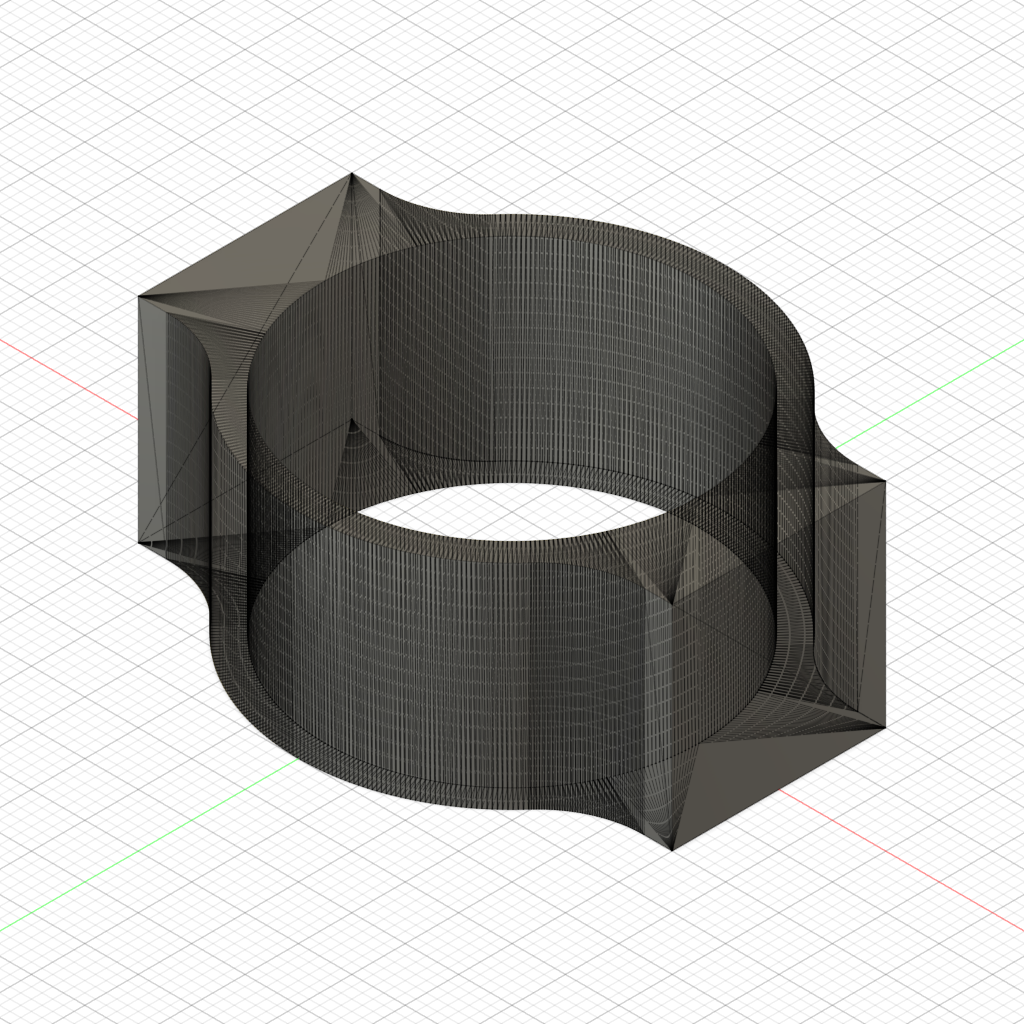
\includegraphics[width=\linewidth]{images/image_demo.PNG} % first figure itself
        \caption*{(a)}
    \end{minipage}\hfill
    \begin{minipage}{0.32\textwidth}
        \centering
        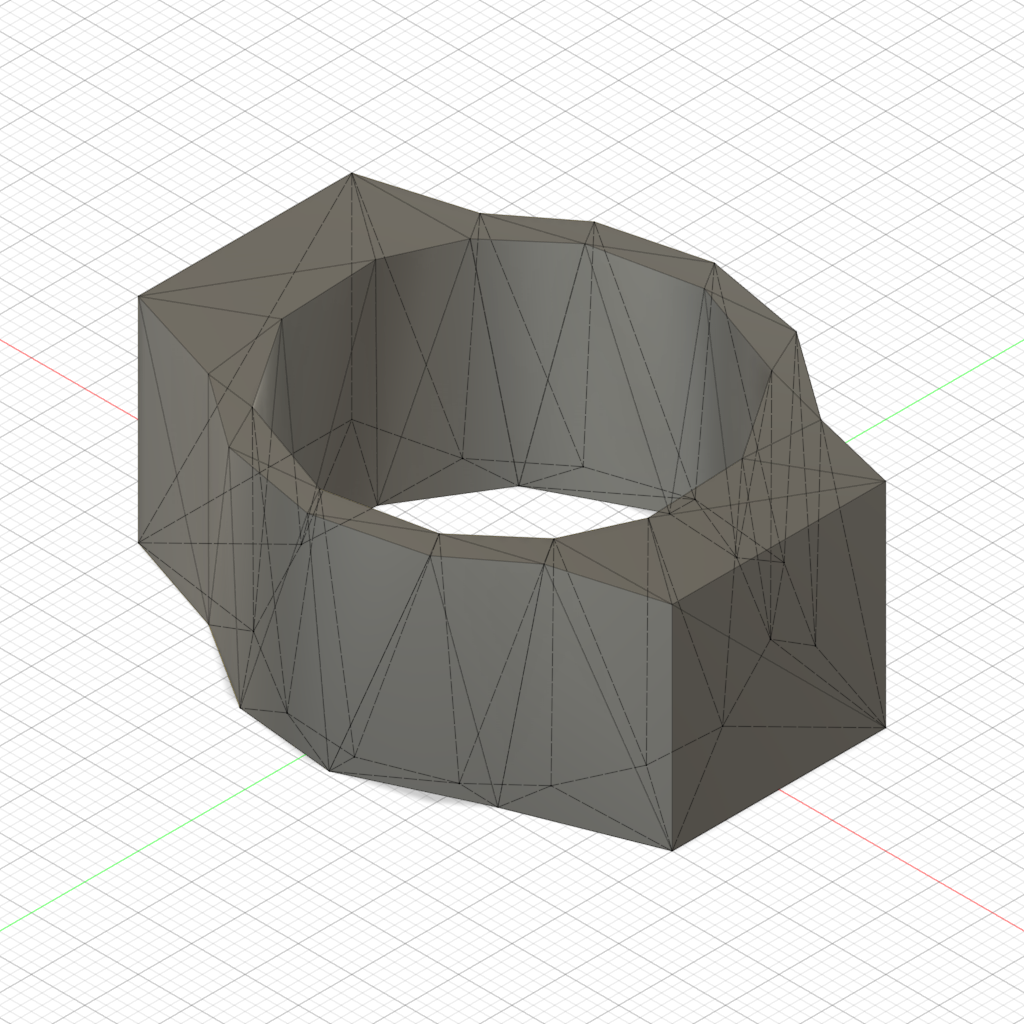
\includegraphics[width=\linewidth]{images/image_demo_medium.PNG} % first figure itself
        \caption*{(b)}
    \end{minipage}\hfill
    \begin{minipage}{0.32\textwidth}
        \centering
        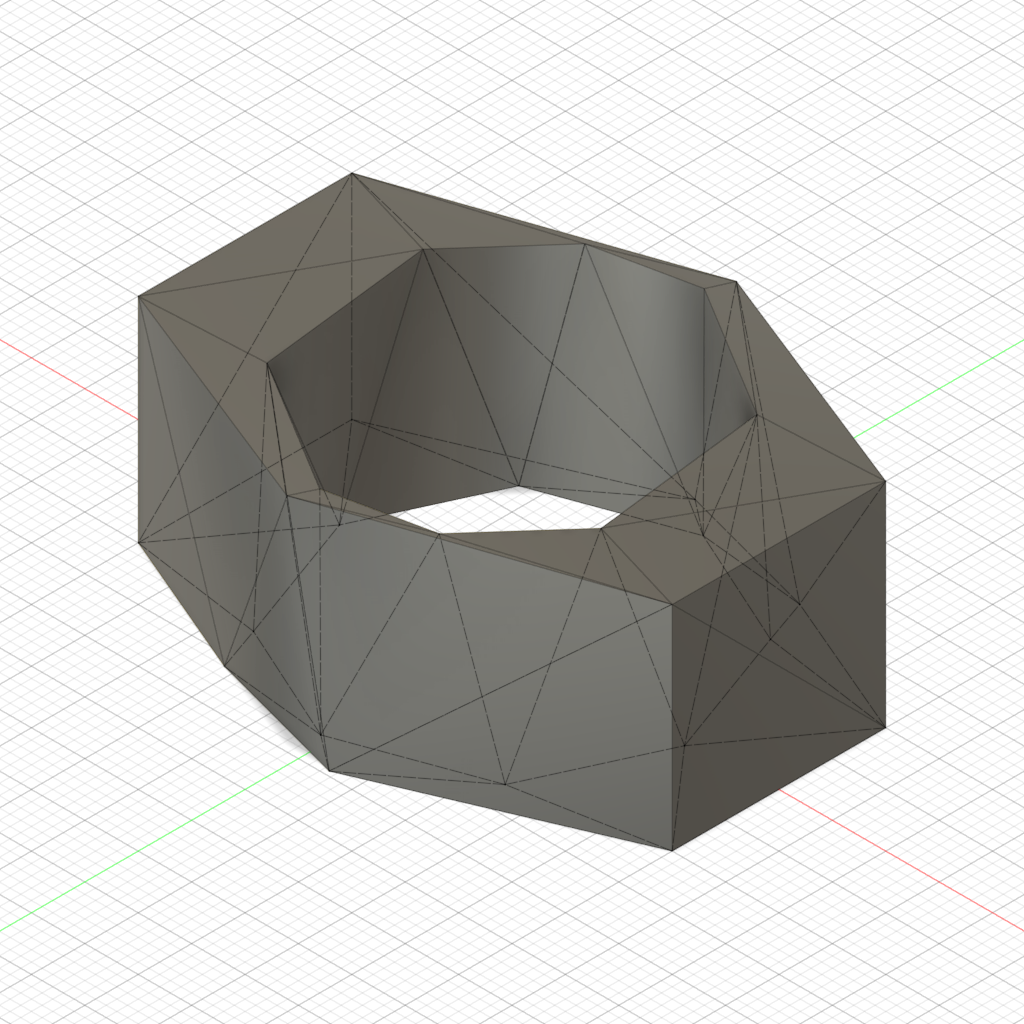
\includegraphics[width=\linewidth]{images/image_demo_low.PNG} % first figure itself
        \caption*{(c)}
    \end{minipage}\hfill

    \caption{Genauigkeit einer 3D-Datei ist abhängig von der Anzahl der gespeicherten
    Eckpunkte am Beispiel des Demonstratorbauteils. (a) 1512 Punkte
    (b) 52 Punkte (c) 30 Punkte}
    \label{fig:3d_design}
\end{figure}

Ein in der akademischen Welt beliebtes Dateiformat für Polygon-Netze ist das 
Polygon File Format (ply).
Das Format kann vom Nutzer beliebig angepasst werden. Eine ply-Datei beginnt mit 
einem Header in dem die Inhaltsstruktur beschrieben wird. 
Für 3D-Objekte besteht diese meistens aus X, Y und Z Koordinaten. 
Zusätzlich können weitere Informationen gespeichert werden. Das ply Dateiformat 
unterstützt standardmäßig: \glqq vertices/edges/faces, vertex colors, textures and
material\grqq ~\cite{KentonMchenry.2008}. Weitere Informationen können durch den Nutzer 
hinzugefügt werden, 
diese können dann aber unter Umständen nicht von anderen Programmen oder Benutzern
benutzt werden.
Im Dateiheader wird zu jedem Attribut auch der Datentyp festgelegt. Durch diesen 
kann die Genauigkeit und Dateigröße beeinflusst werden. Häufig werden hier Floats oder
Integer in verschiedener Bittiefe gewählt.

\section{3D Rekonstruktion} \label{3d_construction}

Bei der Erstellung von digitalen Abbildern geht es nicht nur darum, wie beim Reverse
Engineering, Bauteilgeometrie wieder herzustellen. 3D Modelle bieten auch viele 
Vorteile bei der Analyse von Flächen, Objekten oder sogar Körperteilen. 
Anwendungen sind zum Beispiel in der
geometrischen Dokumentation, Inspektion, Navigation, Visualisierung und 
Objekterkennung zu finden~\cite{Verykokou.2023}. Je nach Anwendungsfall wird eine
bestimmte Genauigkeit
der Daten erwartet, im medizinischen Bereich sind die Ansprüche ganz 
andere als zum Beispiel in der Dokumentierung von ganzen Gebirgszügen.
Das Scannen von Gesichtstexturen zeigte Abweichungswerte zwischen 140 $\mu$m und 
1330 $\mu$m, während die 3D-Rekonstruktion des Kieferknochens Werte zwischen 106 $\mu$m 
und 760 $\mu$m aufwies. 
Bei der digitalen Abtastung von Zahnimplantaten sind die Abweichungen von 
3D Modell und Realität zwischen 19,32 $\mu$m
und 112 $\mu$m groß~\cite{Bohner.2019}.
Bei Lidar-Scans eines Sportkomplexes wurde eine Standardabweichung von ±0.10 Metern
gemessen. Es wurde aus 600 Meter Höhe vermessen und die Scandaten mit 
Referenzpunkten auf dem Boden verglichen.~\cite{Elaksher.2023}
Aus diesem Grund existieren auch verschiedene Herangehensweisen und Technologien  
zur 3D-Rekonstruktion.

3D Rekonstruktion-Technologien können in mehrere Kategorien eingeteilt werden,
bildbasierte Verfahren und  Verfahren die auf Scandaten 
beruhen sind zwei davon.~\cite{Verykokou.2023}
Es existieren auch andere Verfahren die Sensor- oder Volumen-orientiert sind, 
diese nehmen eine Bauteilgeometrie auf, indem ein Sensor das Bauteil abtastet 
und die Berührungspunkte speichert.
Verschiedene Verfahren können auch kombiniert werden, um das endgültige 3D-Modell
realitätsgetreuer zu machen.
Bei bildbasierten Verfahren, auch Fotogrammetrie genannt, wird das 3D Objekt aus
mehreren zweidimensionalen Bildern erstellt, 
umso mehr Bilder vorhanden sind, desto besser kann das
3D Objekt rekonstruiert werden. Um das 3D Objekt zu erstellen werden in 
allen Bildern gemeinsame Punkte gesucht und dann mit der bekannten Kameraposition, 
die relative Position des Punktes im 3D Objekt ermittelt.\cite{schenk2005introduction}
Abbildung \ref{fig:photogammatry} zeigt dies anschaulich.

\begin{figure}[H]
    \centering
    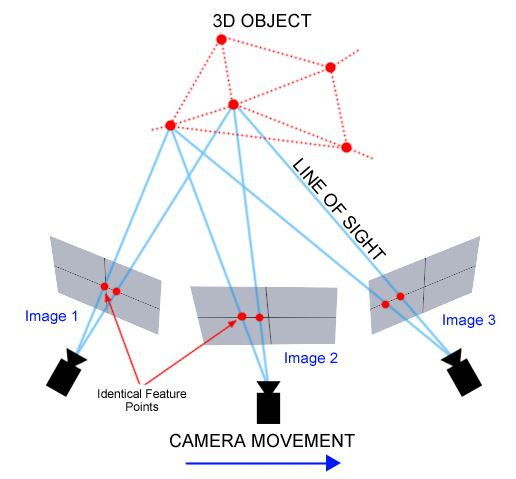
\includegraphics[width=0.7\linewidth]{images/photogrammetry.jpg}
    \caption{Funktionsweise der Fotogrammetrie \cite{.13.08.2024}.}
    \label{fig:photogammatry}
\end{figure}

Vorteil bei der Fotogrammetrie ist, dass die Daten relativ einfach aufgenommen werden
können. Die Kamera eines Smartphones kann ausreichend hochauflösende Bilder aufnehmen, um 
eine 3D-Rekonstruktion zu ermöglichen. Des Weiteren sind viele Softwarelösungen,
auch kostenlose, vorhanden um automatisiert 3D Objekte zu erzeugen.
Gründe, sich gegen den Einsatz von Fotogrammetrie zu entscheiden, 
liegen in der begrenzten Auflösung sowie im signifikant ansteigenden Arbeitsaufwand 
bei steigenden Anforderungen an die Genauigkeit des Endergebnisses. 
Fotogrammetrie zeigt jedoch ihre Stärken bei großflächigen 3D-Rekonstruktionen, 
wie sie beispielsweise bei der Erfassung von Gebäuden, Stadtteilen oder geografischen 
Strukturen erforderlich sind.

%\begin{figure}[H]
%    \centering
%    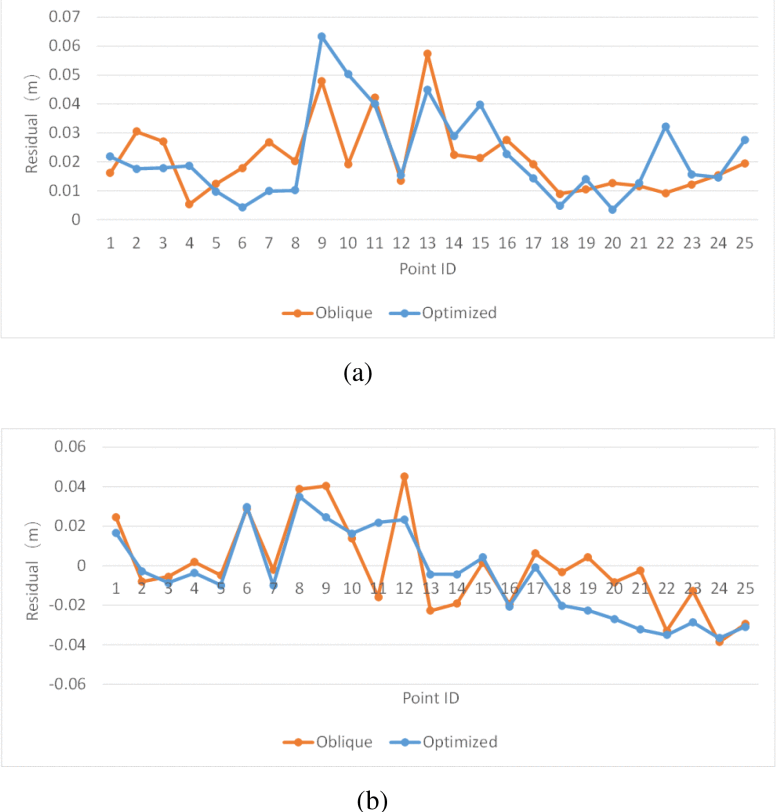
\includegraphics[width=\linewidth]{images/photogammatry_accurancy.PNG}
%    \caption{Genauigkeit der Fotogrammetrie bei Bildern die aus 
%    600 m Höhe aufgenommen wurden \cite{Elaksher.2023}.}
%    \label{fig:photogammatryAccuracy}
%\end{figure}

Für kleine Objekte, bei deren Rekonstruktion eine hohe Genauigkeit gefordert ist, 
sollte daher das Laserscanner basierte Verfahren angewendet werden. Bei diesem Verfahren werden
die Ursprungsdaten dreidimensional mithilfe eines Scanners erfasst. Der Scanner misst dabei, 
meist mithilfe von Lichtstrahlen, den Abstand zu einem Punkt auf dem zu 
rekonstruierenden Objekt. Um eine Vielzahl von Scanpunkten zu erfassen, 
wird entweder das Objekt oder der Scanner bewegt. Je mehr Punkte erfasst werden, 
desto genauer wird das Ergebnis. Allerdings nimmt die Datenmenge mit der Anzahl der 
Scanpunkte ebenfalls zu, was ab einem bestimmten Punkt zu einer Einschränkung durch den 
verfügbaren Speicher führen kann. Zudem steigt die Rechenzeit mit der Datenmenge an, 
und je nach angewendetem Verfahren kann dieser Anstieg sogar 
exponentiell sein~\cite{XiaoleiDu.2009}.

Nachteile von diesem Verfahren sind die hohen initialen Kosten eines Scanners 
und der begrenzte Messbereich. 

\section{Scanner und Datenerfassung} \label{lasers}

Wie in Kapitel \ref{3d_construction} beschrieben, 
können dreidimensionale Daten direkt durch einen Scanner aufgenommen werden. 
Es existieren verschiedene Technologien und Methoden um Scandaten aufzunehmen, 
darunter die schon erwähnte Fotogrammetrie, Laserscanner und 
strukturiertem-Licht-Scanner~\cite{Ruiz.2022}. 
Die Funktionsweise der Scanner sind in Abbildung \ref{fig:scanning_theo} dargestellt.
Der Laserscanner misst die Koordinaten eines Punktes mithilfe der Zeit die zwischen 
Ausstrahlen des Lasers und Ankunft des reflektierten Strahls liegt.
Bei einem strukturiertem-Licht-Scanner wird mithilfe eines Projektors ein Muster 
auf ein Objekt gestrahlt. Durch mehrere Kameras wird dieses Muster auf dem Objekt 
aufgenommen. Je nach Oberfläche wird das Muster, das auf das Objekt gestrahlt, verzerrt.
Diese Verzerrung wird genutzt, um die Oberfläche des Objekts 
abzubilden.~\cite{georgopoulos2010assessing}

\begin{figure}[H]
    \centering
    \begin{minipage}{\textwidth}
        \centering
        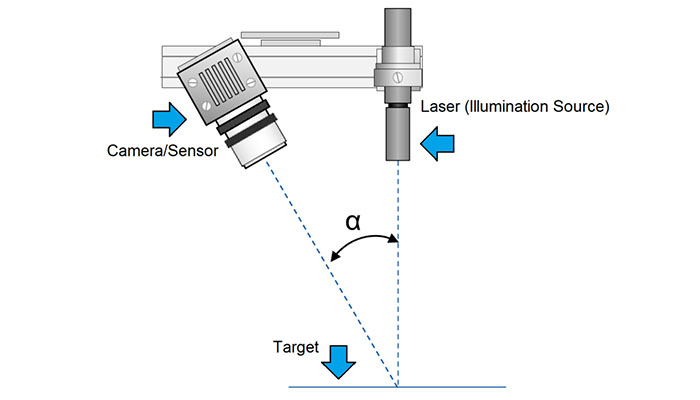
\includegraphics[width=0.8\textwidth]{images/laser_1.jpg} % first figure itself
        \caption*{(a)} 
    \end{minipage}\hfill
    \begin{minipage}{\textwidth}
        \centering
        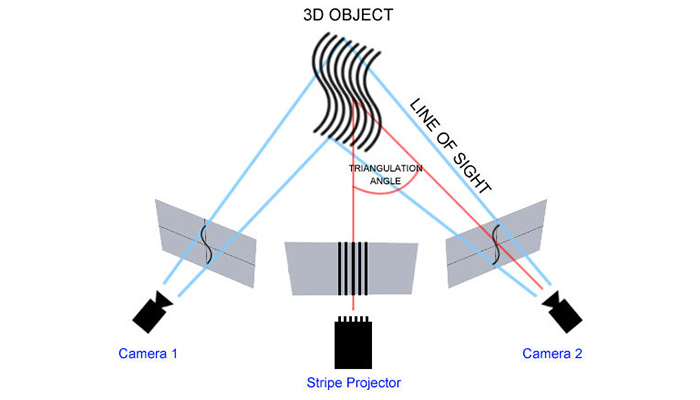
\includegraphics[width=0.8\textwidth]{images/structured_light_1.jpg} % first figure itself
        \caption*{(b)}
    \end{minipage}\hfill
    \caption{Theoretische Funktionsweise von (a) einem Laserscanner und (b) einem 
    strukturiertem-Licht-Scanner~\cite{V..08.08.2019}.}
        \label{fig:scanning_theo}
\end{figure}

Für die Datenerfassung in dieser Arbeit wird ein Laser-Profilsensor verwendet.
Laser-Profilsensoren sind Laser-Scanner, die Höhendaten über 
eine Laserlinie und nicht über einen einzelnen Punkt sammeln. 
Der Scanner hat, abhängig vom Modell und der angebrachten Höhe einen limitierten
Bereich, den er erfassen kann.
In Abbildung \ref{fig:scanner} ist ein Messbereich für den Scanner vom Typ 
ScanControl-LLT30xx sichtbar. Mittig kann 
in einer Tiefe von 85 mm eine Linie mit der Länge 25 mm gemessen werden. 
Der komplette messbare Bereich ist rot markiert. \cite{MESSTECHNIK_2020}

Bauteile die breiter sind als die maximale Breite der Scanlinie, in Abbildung 
\ref{fig:scanner} mittig 25 mm, können also nicht in einem Datensatz erfasst werden. 
Damit eine Digitalisierung von größeren Objekten erfolgen kann, müssen
also mehrere Scans durchgeführt, und später zusammengefügt werden. Zwischen den 
Scanvorgängen muss der Scanner in Richtung der Breitenachse verschoben werden.
Die Länge der Verschiebung sollte kleiner als die Breite der Scanlinie sein, 
damit eine Überlappung entsteht, die 
genutzt werden kann, um die Datensätze wieder zusammenzufügen. Die Verschiebung kann 
beliebig klein gewählt werden, jedoch steigt der Arbeitsaufwand und die Dateigröße mit 
jedem zusätzlichen Datensatz, während das Ergebnis sich nicht verbessert.
Das Ergebnis verbessert sich nicht, da nicht mehr Daten aufgenommen werden, sondern nur 
die gleichen Daten mehrfach.
So können Scandaten aufgenommen werden die dann in dem zu entwickelnde Verfahren
wieder zu einem digitalen Abbild zusammengefügt werden.

\begin{figure}[h]
    \centering
    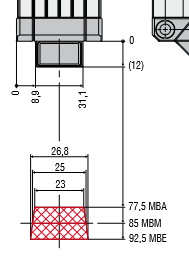
\includegraphics[width=0.3\textwidth]{images/Scanner.PNG}
    \caption{Messbarer Bereich eines Laserscanners vom Typ: ScanControl-LLT30xx.
    Der messbare Bereich ist rot markiert. Die Dimensionen sind in mm angegeben 
    und vom Laserursprung gemessen.}
    \label{fig:scanner}
\end{figure}

\section{Transformationen} \label{Transformation}

Zum Zusammenfügen der Datensätze müssen die Scandaten verschoben werden. 
Diese räumlich Veränderung der Datensätze wird auch Transformation genannt.
Eine Transformation ist eine Funktion, die eine Menge von Punkten in einem
Raum auf eine andere Menge von Punkten in demselben oder einem anderen Raum abbildet. 
Diese Transformationen werden verwendet, um die Lage, Form oder Größe von 
Objekten zu verändern.
Es gibt drei Basis Arten der Transformationen:
Translation, Rotation und Skalierung. Die Translation verschiebt alle Punkte 
um einen bestimmten Vektor in eine bestimmte Richtung. 
Rotation: Drehen eines Objekts um einen Punkt (in 2D) oder eine Achse (in 3D).
Veränderung der Größe eines Objekts durch Multiplikation der Koordinaten 
mit einem Skalierungsfaktor~\cite{XiaoleiDu.2009}.

\section{ICP-Algorithmus} \label{icp}

Eine Möglichkeit zum Zusammenfügen von Datensätze ist der 
Iterative-Closest-Point-Algorithmus (ICP-Algorithmus).
Dieser existiert schon seit dem Beginn der 90er Jahre und ist 
die klassische Methode, wenn es um die Registrierung von Datensätzen geht.~\cite{icp}
Der Algorithmus errechnet eine lokale, optimale Transformation, die ein Daten-Set
dem anderen annähern kann. \cite{icp_og}

Um diese Transformation, zu bestimmen werden zuerst die Distanzen von allen 
Punkten in Daten-Set A zu dem jeweils nächsten Punkt in Daten-Set B aufsummiert 
werden. Dann wird eins der Daten-Sets verschoben und rotiert und wieder die 
Distanzen gebildet. Dies wird so lange gemacht bis die Änderung der Distanzen 
konvergiert. Die entstehende Transformation ist dann optimal.
Für identische Daten-Sets die sich nur in einer Transformation und Rotation 
unterscheiden, funktioniert dieser Algorithmus sehr gut. Bei Daten-Sets die 
Messfehler oder Überlappungen beinhalten kann häufig keine optimale 
Transformation bestimmt werden.
Deswegen wurden seit der ersten Vorstellung des Algorithmus viele Varianzen
entwickelt, die mit diesem Schwächen umgehen. 
Zum Beispiel der 'Sparse Iterative Closest Point' Algorithmus von~\cite{Bouaziz.2013}
oder die 'Anderson-accelerated' Version.
Beide Varianten können besser mit Ausreißern und nur 1
partiell überlappenden Daten umgehen und eine gleichwertige oder bessere 
Transformation, verglichen mit dem originalen ICP-Algorithmus, errechnen.\ \cite{icp}

Der Algorithmus geht iterativ vor und berechnet immer eine optimale lokale Transformation.
Die beiden Daten-Set sollten schon vor dem Anwenden des ICP-Algorithmus grob angenähert sein, 
das beschleunigt die Konvergenz und damit die Laufzeit des Algorithmus.
Eine grobe Annäherung kann ermittelt werden, indem die Massenmittelpunkte der beiden Daten-Set
übereinander gelegt werden. In Abbildung \ref{fig:ipc_princip} ist das Prinzip visuell 
dargestellt. Die grünen Linien sind jeweils die kürzeste Distanz von Q nach P. 

\begin{figure}[h]
    \centering
    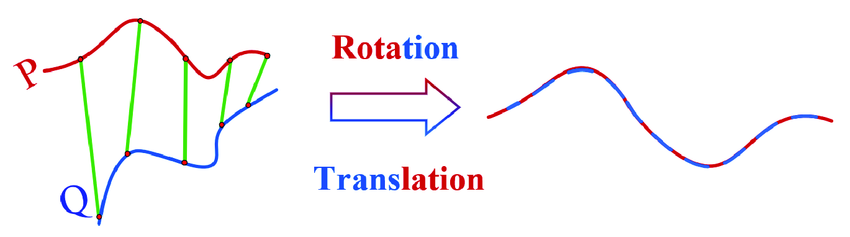
\includegraphics[width=0.9\textwidth]{images/Principle-of-ICP-algorithm.png}
    \caption{Prinzip des ICP-Algorithmus~\cite{icp_img}}
    \label{fig:ipc_princip}
\end{figure}

